\documentclass[tikz,border=10pt]{standalone}
\usepackage{tikz}
\begin{document}
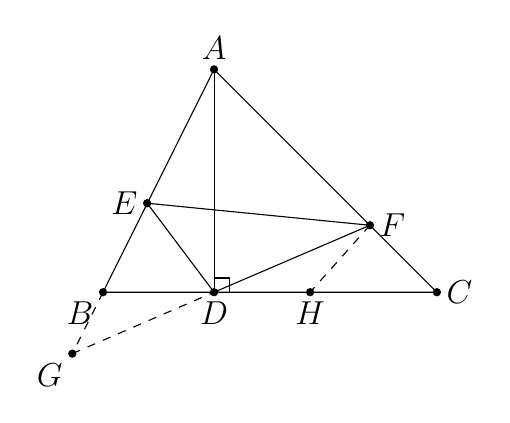
\begin{tikzpicture}[scale=1, every node/.style={font=\large}]
  \coordinate (A) at (2.58,2.83);
  \coordinate (E) at (1.73,1.13);
  \coordinate (B) at (1.17,0);
  \coordinate (D) at (2.58,0);
  \coordinate (H) at (3.80,0);
  \coordinate (C) at (5.41,0);
  \coordinate (F) at (4.56,0.85);
  \coordinate (G) at (0.78,-0.78);

  % solid edges
  \draw (A) -- (B) -- (C) -- cycle;
  \draw (A) -- (D);
  \draw (E) -- (D) -- (F);
  \draw (E) -- (F);

  % dashed edges
  \draw[dashed] (B) -- (G);
  \draw[dashed] (G) -- (D);
  \draw[dashed] (F) -- (H);

  % right angle mark at D
  \draw (2.58,0) -- (2.58,0.18) -- (2.78,0.18) -- (2.78,0);

  % points
  \fill (A) circle (1.5pt);
  \fill (E) circle (1.5pt);
  \fill (B) circle (1.5pt);
  \fill (D) circle (1.5pt);
  \fill (H) circle (1.5pt);
  \fill (C) circle (1.5pt);
  \fill (F) circle (1.5pt);
  \fill (G) circle (1.5pt);

  % labels
  \node[above] at (A) {$A$};
  \node[left] at (E) {$E$};
  \node[below left] at (B) {$B$};
  \node[below] at (D) {$D$};
  \node[below] at (H) {$H$};
  \node[right] at (C) {$C$};
  \node[right] at (F) {$F$};
  \node[below left] at (G) {$G$};
\end{tikzpicture}
\end{document}
